\documentclass[12pt]{article}

\usepackage[slovene]{babel}
\usepackage[top=1in, bottom=1in, left=1in, right=1in]{geometry}
\usepackage{graphicx}
\usepackage{caption}
\usepackage[hidelinks,unicode]{hyperref}
\usepackage{tikz}
\usepackage{tikz-timing}
\usepackage{amsmath}
\usepackage[utf8]{inputenc}
\renewcommand{\contentsname}{Kazalo}
\renewcommand\listfigurename{Kazalo slik}
\renewcommand{\figurename}{Slika}
\usepackage{listingsutf8}

\begin{document}
\pagenumbering{gobble}
\linespread{1.25}
\begin{titlepage}
  \begin{center}
    
\includegraphics[height=2cm]{slike/vegova.png}\\
    \Huge
    \vspace*{6cm}
    Raziskovanje mej RISC-a\\
    \Large
    (računalništvo in informatika)\\
    Raziskovalna naloga\\
  \end{center}
  \vspace{8cm}
  \begin{tabular}{rl}
    Avtor: & Adrian Sebastian Šiška\\
    Mentor: & Aleš Volčini
  \end{tabular}
  \vspace{1cm}
  \begin{center}
    Ljubljana, marec 2022
  \end{center}
\end{titlepage}

\pagebreak
\pagenumbering{arabic}

\tableofcontents

\pagebreak

\listoffigures

\pagebreak

\section{Zahvala}
Zahvaljujem se vsem, ki so mi pomagali pri raziskovanju in pisanju.
Še posebej se zahvaljujem mentorju Alešu Volčiniju za podporo in potrpežljivost.
Zahvalil bi se tudi mojima prijateljema Oliverju Wagnerju (\url{oliwerix.com}) in Antonu L. Šijancu (\url{sijanec.eu}), ki sta z implementacijami svojih emulatorjev popestrila moje delo.

\pagebreak

\section{Povzetek}
V raziskovalni nalogi sem si zamislil novo RISC arhitekturo, imenovano MUHI (\textit{Minimal URISC hardware implementation}).
MUHI je enobitna, dvo-instrukcijska arhitektura.
Za njeno implementacijo sem raziskoval področje teorije izračunljivosti in arhitekture ostalih procesorjev.
Za testiranje delovanja sem sprogramiral emulator, za lažje pisanje programov pa sem pripravil tudi zbirnik in razbirnik.
Kot pomoč pri iskanju sestavljenih operacij sem napisal še program za iskanje kombinacij ukazov.
Implementacija je Turing-kompletna, kar sem dokazal tako, da sem napisal celični avtomat, ki izvaja pravilo 110.

Ključne besede: RISC, URISC, arhitektura procesorja, Univerzalen procesor, navidezna naprava, emulacija

\pagebreak

%% ANG ONLY DEU
% \section{Abstract}

\section{Uvod}
Procesorji so najpomembnejša komponenta v moderni zgradbi računalnika, kljub temu, jih ljudje dandanes čedalje slabše razumejo.
Oblikovanje procesorjev smo prepustili drugim procesorjem, z nizkimi jeziki se pa še malokdo ukvarja.
To me čudi, saj vse od kar sem slišal za Intelov \textit{management engine} ne morem nehati razmišljati o mojem procesorju.
Spraševati sem se začel, kako lahko zares preverim, da management engine ni aktiven v mojem računalniku in ali lahko sploh zaupam svojemu procesorju.
Edini zadovoljiv odgovor, ki sem ga do sedaj našel je, da naredim svoj procesor.
Tako sem si zamislil MUHI arhitekturo.

\subsection{Hipoteza}
V tej nalogi bom preveril resničnost sledeče hipoteze:
\begin{itemize}
  \item Moja lahkotna arhitektura imenovana MUHI je Turing complete.
\end{itemize}

\section{Moja arhitektura}
\begin{center}
  %cd slike ; dot -O -Tpdf arhitektura.gv; cd ..
  \includegraphics[width=.5\linewidth]{slike/arhitektura.gv.pdf}
  \captionof{figure}{Shematika MUHI-ja}
\end{center}
Imenuje se \textit{Minimal URISC hardware implementation} oz.\ kratica MUHI.\@
\subsection{Kaj je URISC?}
% URGENTLY religate interesting stuff to the compiler
Kratica URISC pomeni \textit{ultimate reduced instruction set computer}, kar bi lahko v slovenščino prevedli kot \textit{računalnik z dokončno zmanjšano množico operacij}.
RISC arhitekture so v praksi, odkar pomnilnik ni več drag, boljše od CISC arhitektur, to nam dokazujejo moderni pametni telefoni, saj skoraj vsi delujejo na ARM čipih.
To nam dokaže tudi najpopularnejši ustvarjalec CISC procesorjev, Intel, saj so dandanes njihovi procesorji interno zgrajeni iz tolmača in manjšega RISC procesorja.
Da arhitekturo označimo kot URISC, pa moramo iti še korak dajle in se znebiti vsek ukazov, razen enega.
Zanimiva posledica tega je dejstvo, da lahko, ko pišemo strojno kodo popolnoma spustimo polje z instrukcijo, ostanejo le še njeni argumenti.

V virih najdemo primere ukazov, ki so sami po sebi Turing complete, npr.\ x86 mov ukaz.
Jaz sem se raje odločil za 2 instrukciji, ker se njuni rabi ne prekrivata zelo dosti, saj med drugim tudo operirata na različnih magnitudah količine podatkov. Posledica tega dodatka je lažje pisanje programov.
Odločil sem se, da mi je težavnost pisanja programov brez prevajalnika pomembna, ker bi sicer ta naloga vzela še dosti več časa, če bi moral napisati še prevajalnik.

\subsection{Instrukcije}
Obe instrukciji prejmeta 2 naslova iz rama\footnote{naslov ni nujno povezan z ramom, glej \textit{c16} instrukcijo} in en meta bit.
V moji izvedbi sem se odločil za 7-bitne\footnote{Ta izbira je arbitrarna, arhitektura podpira $n$ bitne naslove. Tega sem izbral, ker je posledična dolžina ukaza v bitni kodi potenca števila 2.} ram naslove.
Za pridobivanje bitnega zapisa preprosto napišemo 1.\ naslov, 2.\ naslov, cifro željene instrukcije in meta bit.
Meta bit je nastal zaradi poravnave dolžine ukaza na 2 bajta, s čimer je naredilo pisanje zbirnika in razbirnika nekoliko lažje.
Obe instrukciji se obnaša tako, da vzameta podatke iz 1.\ naslova in rezultat shranita na 2.\ naslov.

\subsubsection{Instrukcija ``c16''}
To je 1.\ instrukcija, označena z 0 v binarni obliki.
Njena notacija izhaja iz daljšega imena \textit{copy 16 bits}
Deluje tako, da od njenega 1.\ podanega naslova in še zaporedno naslednjih 15 registrov prekopira v začasen pomnilnik, potem pa jih prekopira na 2.\ naslov in na zaporednih 15 registrov za njim.
Odločitev, da bo to 1.\ instrukcija, izhaja iz tega, da so same ničle v programu interpretirane kot ukaz brez posledic, kar je uporabno predvsem takrat, ko je potrebno z ničlami rabim kaj poravnati na naslov, ki je par mest nižje.
Na začetku je bila zasnovana skoraj kot jump instrukcija, saj z NANDom ni mogoče vseh bitov v programskem števcu hkrati spremeniti na željeno vrednost.
Posledica spremembe enega pa po enega bita v programskem števcu, bi bil skok takoj po 1.\ spremembi enega bita, saj kontrolna enota vedno preveri števec pred nalaganjem nove instrukcije.

Ko sem kasneje dodal še meta bit, sem se odločil, da se bo kopiranje ob nastavljenem meta bitu zgodilo iz programskega spomina.
S tem je nalaganje konstant, kot so nizi ali pa naslovi funkcij, postalo zelo preprosto in hitro.
Omejitev tega je, da sem uporabil 7 bitni naslov za pridobivanje podatkov iz pomnilnika opisanega s 16 biti.
Zaradi tega večina pomnilnika še vedno ni na voljo, kot rešitev temu pa sem se odločil, da sem uporabil skrite registre kot nastavitev strani programskega pomnilnika.

Skriti biti nastanejo kot stranski učinek slabe definicije zaporednih registrov.
Kaj se zgodi, če nekaj skopiramo na zadnji register?
Zdi se mi, da je najbolj uporaben odgovor, da rečem, da so za \textit{zadnjim registrom} še \textit{skriti registri}.
Do njihove vsebine se da dostopati le s \textit{c16} ukazom, kar se mi ne zdi problem, saj menim, da bo ta konfiguracija redko spremenjena med potekom programa.

Torej se ukaz \verb|c16 0x22, 0x44, 0| prevede v \verb|0100010 1000100 0 0|, kar bi lahko predstavili s Cejevsko vrstico kode\\
\verb|int *a=0x22; int* b=0x44; *b=*a;*(b+1)=*(a+1)|\ldots \verb|*(b+15)=*(a+15)|.

\subsubsection{Instrukcija ``Nox''}
To je 2.\ instrukcija, označena z 1 v binarni obliki.
Ime izhaja iz njenega kratkega opisa: \textit{NAND or XOR}.
Najprej sem poizkusil uporabiti le XOR, kot edini ukaz za minpulacijo bitov, vendar sem hitro ugotovil, da se iz samo XORa ne da rekonstuirati vseh ostalih logičnih vrat.
Zato sem se odločil še za najpogosteje izbrana univerzalna vrata NAND.\@

Ta so s seboj privlekla nove probleme; npr.\ pogojni skoki naprej so postali zelo dragi.
Programski števec bi bil lahko viden samo c16 ukazu, vendar bi to preprečilo relativne skoke, kjer spremenim le 1 bit v njem.
Pogojni relativni skoki so nadaljevanje tega. Ker vem, kje se nahaja trenuten ukaz, lahko vem, v kakšnem stanju je nek bit v programskem števcu.
S kombiniranjem enice v programskem števcu in nekega podatka v ramu lahko skočim nazaj samo takrat, ko je tudi podatek v ramu enica.
Pogojen skok naprej ni izvedljiv na tak način, saj bo na enobitnem mestu, če ga želimo povečati, morala biti ničla.
NAND pravi, da, če je kateri koli izmed argumentov 0, da bo rezultat vedno 1, kar pomeni, da naš \textit{pogoj} ni bil upoštevan.

Zaradi dragih skokov in lahke ponastavitve celice na 0, sem se odločil, da dodam še XOR.\@
Par vrat sem kombiniral v eno instrukcijo, kjer meta bit izbira med njima.

\begin{displaymath}
  f(A,B,M) =
  \begin{cases}
    NAND(*A\footnote{*N pomeni priklic iz rama z naslovom N}, *B) \rightarrow *B & M=0\\
    XOR(*A, *B) \rightarrow *B & M=1
  \end{cases}
\end{displaymath}
Oz.\ zapisano v logični notaciji.
\begin{displaymath}
  \overline{(AB)}(A+B+\overline{C})
\end{displaymath}

Torej se ukaz \verb|Nox 0x15, 0x53, 0| prevede v \verb|0010101 1010011 1 0|, kar bi lahko predstavili s Cejevsko vrtico kode \verb|int *a=0x15;int *b=0x53;*b=NAND(*a,*b)|.

\subsection{Enobitni registri}
% vsi registri so eneaki, samo eni so bol enaki
Kot ram sem si zamislil \textit{trak} enobitnih registrov.
Zaradi preprostosti, je programski števec preslikan čez prvih 16 registrov, da lahko tudi ukaz \textit{Nox} z njim operira.
Ves I/O je prav tako preslikan na registre, in sicer na prve štiri za števcem.
Število vseh registrov je funkcija dolžine naslova rama in velikosti programskega števca.
Velikost programskega števca je potrebno upoštevati, saj je glede na njo definiran ukaz za kopiranje, kot polsedica ukaza za kopiranje so definirani skriti registri.
Za računanje dolžine traka registrov sem pripravil preprosto formulo.
$F(N,P)$, v mojem primeru $F(7,16)$, izračuna število registrov, ki jih imam na razpolago, pri danem N in P.
\begin{center}
  \begin{displaymath}
    F(N,P)=2^{N}+P-1
  \end{displaymath}
  $F(N,P)$ je število registrov, $N$ je dolžina binarnega naslova, $P$ je dolžina programskega števca
\end{center}

\subsection{Komunikacija z zunanjim svetom}
Za izvedbo vhodno-izhodnih operacij, se odločil da bom implementirati svojo 4 žično komunikacijo.
Ta lahko asinhrono bere informacije po bitih.
Asinhronost je pomembna lastnost, saj nimam nikjer prostora, kamor bi dodal začasen pomnilnik, ki bi shranjeval podatke, preden bi procesor imel čas, da se začne ukvarjati z njimi.

Interrupt tudi ni dobro nadomestilo asinhronosti, saj bi dodal ogromno kompleksnosti, kot npr.\ najmanj 16 dodatnih registrov, instrukcijo za branje z njih, in možnost spreminjanja registrov, ki ni posledica nekega ukaza.
Lepa lastnost štirižičnega protokola je tudi, da se dve napravi z lahkoto skupaj poveže, saj moramo le izhode iz ene priklopti v vhode druge.
\begin{center}
  \begin{tabular}{ccc}
    $A_{OUT}  $ & \texttiming{LHHHLLLLLL} & $B_{IN}$\\
    $A_{OUT_A}$ & \texttiming{LLHZLLLLLL} & $B_{IN_A}$\\
    $A_{IN}   $ & \texttiming{LLLLLHHHHL} & $B_{OUT}$\\
    $A_{IN_A} $ & \texttiming{LLLLLLHZLL} & $B_{OUT_A}$
  \end{tabular}\footnote{modra črta na sredini prikaže stanje, kjer ena naprava drži signal pri logični enici, druga naprava pa ga poizkuša nastaviti na ničlo}

  \text{Primer pošiljanja enice od A do B in od B do A}
\end{center}
Za pošiljanje informacij najprej počakaš, da je $OUT_{A}$ dovoljen, torej 0.
Nato lahko pišemo, kar hočemo, v $OUT$, dokler ne želimo vrednosti \textit{oddati}, kar naredimo s tako, da napišemo enico na $OUT_{A}$.

Za prejemanje informacij je postopek podoben.
Začnemo s preverjanjem $IN_{A}$, kot da bi gledali nabiralnik, če nam je poštar kaj prinesel.
Čim dobimo napisano enico, smemo interpretirati karkoli je trenutno v $IN$, kot podatke.
Da dobimo naslednji znak, priklopimo pulldown upor na $IN_{A}$.
To druga naprava zazna in čim prej spusti $IN_{A}$ na 0.


\section{Izdelava}
Za uspešno izdelavo sem se odločil da bom potreboval okolje, kjer lahko testiram spremembe arhitekture in moje programe.
Zato sem se lotil pisanja virtualnega stroja, ker pa je težko vedeti, če zares deluje, sem začel delo na zbirniku, da mi ne bi bilo več treba na roke pisati enic in ničel.
Seveda je izdelava zbirnika tudi težka, zato sem razvil še razbirnik, da preverim delovanje zbirnika.
Izdelava le tega je bila nekoliko lažja, kljub temu sem čez nekaj dni našel večjo napako pri de dekodiranju ukazov.

\subsection{Zbirnik (assembler)}
Glej prilogo \textit{asm.py}.

Najprej celotno datoteko podamo NASMovemu prepreprocesorju.
Potem za vsako vrstico v datoteki:
\begin{itemize}
  \item preiščemo vrstico za par ``$<py>$'' simbolov, ki tvorita python blok.
  Vsaka uporabnikova konstanta je tako ali tako interpretirana skozi oči pythona, vendar nastane problem, ko želimo interpretirati pythonov izraz, ki vsebuje vejice.
  Vejice so namreč ločilo med polji, zato moj preprost razpoznavalnik nepravilno nareže en pythonov izraz na več majhnih delov, ki sami po sebi niso več veljavni.
  \item Na koncu vse py bloke zamenjamo z njigovimi izračunanimi vrednostmi v vrstici.
  \item Nato klasificiramo vsako vrstico v eno izmed petih možnih vrst.
  \begin{itemize}
    \item Komentar ali prazna vrstica, ki jo lahko varno spustimo,
    \item Surovi binarni podatki, ki jih direktno zapišemo v datoteko,
    \item Premik v programu: premaknemo mesto pisanja in nadaljujemo,
    \item Instrukcija v procesorju, ki jo dekodiramo, izračunamo njene argumente in zapišemo,
    \item Naslov, katerega pozicijo si zapomnimo, da bomo kasneje lahko omenjali predmet pred katerim stoji.
  \end{itemize}
\end{itemize}

\subsubsection{Preprocessor}
Preprocessor skrbi za dodajanje večih datotek skupaj in dešifriranje makrotov ter definicij.
Program \textit{NASM} je precej popularen zbirnik, ki mi dovoli, da z lahkoto uporabim le njegov preprocesor.
Ker moramo zaradi oblike zbirnega jezika ohraniti vrstice iz izvorne kote, C-jev preprocesor ni primeren.

\subsection{Razbirnik (Dissasembler)}
Glej prilogo \textit{disasm.py}.

\begin{center}
  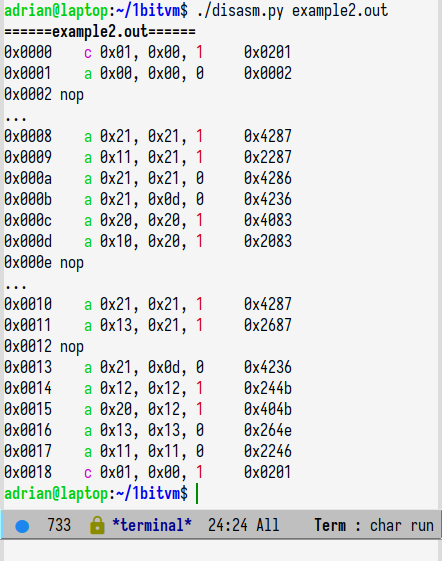
\includegraphics[width=.3\linewidth]{slike/razbirnik.png}
  \captionof{figure}{Primer uporabe razbirnika}
\end{center}
Med izdelavo delujočega zbirnika sem naletel na nekaj problemov, zato sem z malo pomoči Oliverja napisal še manjši program, ki se sprehodi čez datoteko in jo interpretira v instrukcije in njene argumente.
Izpiše nam naslov, na katerem se ukaz nahaja, ukaz sam, meta bit in še šestnajstiški prikaz tega ukaza, saj ne loči med podatki in ukazi.

\subsection{Iskanje ukazov s surovo silo}
Glej prilogo \textit{gate-bf}.
Pisanje makrotov, kot so \texttt{add} je človeku zelo težko opravilo.
Seveda se da najti kombinacijo NAND-ov in XOR-ov, ki bi mi vrnila seštevek dveh številk, vendar ne morem biti prepričan, da sem res našel najkrajši algoritem za to.
Zato sem napisal program, ki najde najkrajše kombinacije ukazov namesto mene in jih zapiše v tabelo.
V taki tabeli poiščeš mesto z številskim opisom tvojega problema, in prepišeš zaporedje ukazov, ki reši tvoj problem.
Ideja je v tem, da za vsak možen vhod v $n$ celic poizkusimo vse možne ukaze, in gledamo, kdaj dobimo nov rezultat.
Ko dobimo kaj novega, lahko preprosto ponovimo postopek.
Tako lahko generiramo tabelo rezultatov glede na vse možne vhode.

Prva implementacija tega programa je bila napisana v pythonu in bi po mojih ocenah trajalo nekaj tednov, da bi dobil popolno tabelo vseh možnih rezultatov.
Zato sem prepisal cel program v C in z uporabo več niti hkrati, skrajšal čas iskanja na 3 sekunde.

\section{Virtualna implementacija}
Glej prilogo \textit{main.py}.
Da zares lahko pokažem delovanje naprave, moram nekako prikazati kako deluje, in to na najlažji način dosežem z implementacijo v virtualnem okolju.
Zato sem se lotil pisanja virtualne naprave v pythonu.
Svoji 2 izhodni žici ima povezani na standardni izhod, svoji 2 vhodni žici pa na standardni vhod.
Tako lahko preko terminala komuniciramo z navidezno napravo.
To lahko najlažje vidimo pri 1.\ primeru, kjer naprava izpiše ``Zivjo'', ali v 2.\ primeru, kjer nam naprava vrne nazaj vsak bit, ki ga prejme.
\subsection{Celični avtomat}
\begin{center}
  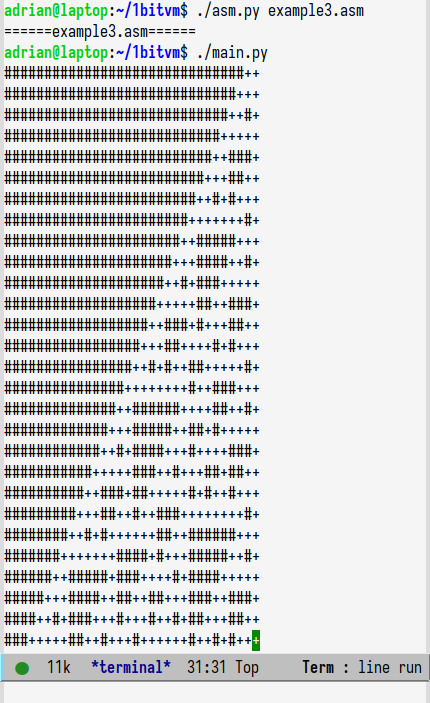
\includegraphics[width=.3\linewidth]{slike/pravilo110.png}
  \captionof{figure}{Prikaz delovanja celičnega avtomata na MUHI arhitekturi.}
\end{center}
Kot metodo dokazovanja, da je MUHI Turing complete, sem izbral emulacijo drugega Turing complete sistema.
Eden izmed najbolj preprostih, čeprav še vedno dovolj kompleksnih, da je univerzalen, je Celični avtomat s pravilom 110.
Seveda ne morem implementirati neskončno dolgega enodimenzionalnega traka, na katerem bi simuliral izvajanje tega pravila, lahko pa pokažem, da bi se to dalo implementirati, če bi moja naprava imela neskončno rama.

\section{Zaključek}
\subsection{Hipoteza}
\begin{itemize}
  \item Moja lahkotna arhitektura imenovana MUHI je Turing complete.
  Hipoteza potrjena, saj lahko popolnoma emulira sistem, za katerega je že bilo dokazano, da je Turing complete
\end{itemize}

\section{Nadaljne raziskave}
Zdi se mi pomembno omeniti, da lahko ob ohranitvi preprostosti dizajna moje enobitne arhitekture močno razširimo njeno moč tako, da jo uporabimo kot generator programskega spomina sebe.

\section{Priloge}

Vse priloge in izvorna koda so dosegljive na \url{https://github.com/adimineman/raziskovalna} in so licencirane z odprtokodno licenco.

\lstset{
  basicstyle=\footnotesize,
  breaklines=true,
  frame=single,
  stepnumber=5,
}
\lstdefinestyle{py}{
  language=Python,
}

\lstdefinestyle{asm}{
  language=[x86masm]Assembler,
  morekeywords={copy, nand, xor, x, a, c},
}
\lstdefinestyle{cst}{
  language=C,
}

\lstinputlisting[style=py,caption=asm.py]{1bitvm/asm.py}
\lstinputlisting[style=py,caption=disasm.py]{1bitvm/disasm.py}
\lstinputlisting[style=asm,caption=example.asm]{1bitvm/example.asm}
\lstinputlisting[style=asm,caption=example2.asm]{1bitvm/example2.asm}
\lstinputlisting[style=asm,caption=example3.asm]{1bitvm/example3.asm}
\lstinputlisting[style=asm,caption=std.asm]{1bitvm/std.asm}
\lstinputlisting[style=py,caption=main.py]{1bitvm/main.py}
%\lstinputlisting[caption=Primer razporeditve pomnilnika]{1bitvm/mem}
\lstinputlisting[style=py,caption=oneb\_vm.py]{1bitvm/main.py}
\lstinputlisting[style=cst,caption=gate-bf]{gate-bf/main.c}

\pagebreak
\section{Viri in literatura}
$[1]$ Andreas Abel, upops.info: Characterizing Latency, Throughput, and Port Usage of Instructions on Intel Microarchitectures, ACM, 2019, dosegljivo: \url{https://uops.info/} [23.3.2022]\\
$[2]$ Crystal Chen, RISC architecture, 2000, dosegljivo: \url{https://cs.stanford.edu/people/eroberts/courses/soco/projects/risc/risccisc/} [23.3.2022]\\
$[3]$ Matthew Cook, Universality in Elementary Cellular Automata, Department of Computation and Neural Systems, 2004, dosegljivo: \url{https://wpmedia.wolfram.com/uploads/sites/13/2018/02/15-1-1.pdf} [23.3.2022]\\

% \pagebreak
% \section{Viri slik}
\end{document}
